% Certificador: componente de PPA que "certifica" las demostraciones,
%     generando un certificado en deducción natural. Implicó escribir muchos
%     meta-teoremas.
%     \begin{itemize}
%         \item Formalización de muchos teoremas y axiomas: contextos (vale en el prefijo)
%         \item Proof y proof steps, simplificación de la interfaz y mapeo de
%         comandos a steps
%         \item Implementación de cada comando
%         \item By y solver para resolver varios. DNF. Extensión con foralls
%         consecutivos. Demostración / justificación de que es correcto y completo
%         para LP, pero heurístico para LPO (mostrar un caso en el que no funcione)
%         \item Descarga de conjunciones
%         \item Uso de dneg elim como razonamiento por el absurdo para demostrar
%         deMorgan y equivalencias.
%     \end{itemize}

En la sección anterior vimos cómo usar PPA para demostrar teoremas. Pero, ¿cómo
funciona por detrás? ¿Como asegura la validez lógica de las demostraciones
escritas por el usuario?

\section{Certificados}

Los programas de PPA se \textbf{certifican}, generando una demostración en
deducción natural. ¿Por qué? El lenguaje de PPA es complejo, la implementación
no es trivial. Si se escribe una demostración, para confiar en que es correcta
hay que confiar en la implementación de PPA.

Pero si PPA genera una demostración de bajo nivel, que usa las reglas de un
sistema lógico simple y conocido, entonces cualquiera que desconfíe
podría fácilmente escribir un chequeador, o usar uno confiable. Por eso genera
demostraciones en deducción natural, haciendo que cumpla con el \textbf{criterio
de de Bruijn}

\begin{definition}[Criterio de de Bruijn \cite{freek-bruijn}] Un asistente de
    demostración que satisface que sus demostraciones puedan ser chequeadas por
    un programa independiente, pequeño y confiable se dice que cumple con el
    criterio de de Bruijn.
\end{definition}

El módulo de PPA que \textit{certifica} las demostraciones de alto nivel de PPA
generando una demostración en deducción natural es el \modCertifier{}. Si
bien toda demostración que genere debería ser correcta, para atajar posibles
errores siempre se chequean con el \modChecker{} de DN.


\duda{Para pablo: pero si emite certificados que no corresponden a la demo original y chequean siempre, por ej. siempre el mismo, no estaría mal igual? Tenés que confiar también en la parte que emite el certificado.}

\section{Certificador}

El \modCertifier{} en realidad no genera una sola demostración de deducción
natural, sino que al poder haber más de un teorema en un archivo PPA, este
genera un \textbf{contexto} compuesto por una lista ordenada de
\textbf{hipótesis}. Hay dos tipos

\begin{itemize}
    \item Teoremas: son fórmulas con demostraciones asociadas.
    \item Axiomas: son fórmulas que se asumen válidas (pueden ser usadas para
    modelar una teoría)
\end{itemize}

\begin{figure}[H]
    \centering
    \begin{multicols}{2}
        \begin{tabular}{c}
            \lstinputlisting{listings/certifier/two-theorems.ppa}
        \end{tabular}
        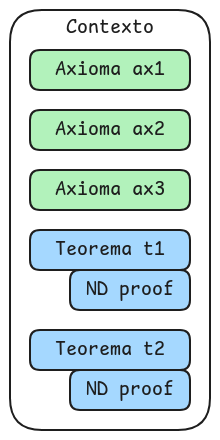
\includegraphics[scale=0.5]{img/ppa-context.png}
    \end{multicols}
    \caption{Contexto resultante de certificar de un programa}
\end{figure}


Por lo tanto, en vez de chequear demostraciones, se chequean contextos: Una
demostración será válida en el \textit{prefijo estricto del contexto} que la
contiene. Es decir, a la hora de chequearla, se deben asumir como ciertas todas
las hipótesis que fueron definidas previamente.

Pero no solo los axiomas y teoremas declarados en el programa se agregan al
contexto. Cada demostración de un teorema tendrá además un \textit{contexto
local} que extiende al anterior, solo en el marco de su demostración. Las
afirmaciones auxiliares que no afectan la tesis (\lstinline{have},
\lstinline{claim}, \lstinline{consider}, etc.) se agregan como teoremas. Por lo
tanto, cuando se citen, se pegan sus demostraciones. Por otro lado, algunos
comandos agregan axiomas, los mismos que en deducción natural agregan fórmulas
al contexto (\lstinline{suppose} y \lstinline{consider}). Es correcto asumir
como ciertas esas hipótesis, porque lo mismo se hará durante el chequeo de la
demostración en deducción natural.

\begin{figure}[H]
    \centering
    \begin{multicols}{2}
        \begin{tabular}{c}
            \lstinputlisting{listings/certifier/local-context.ppa}
        \end{tabular}
        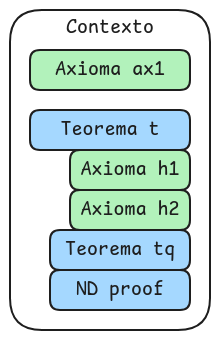
\includegraphics[scale=0.5]{img/ppa-local-context.png}
    \end{multicols}
    \caption{Contexto local}
\end{figure}

\section{Funcionamiento del by}

El \lstinline{by} es el mecanismo principal de demostración en PPA, y el corazón
del \modCertifier. Muchas funcionalidades están implementadas a su alrededor.
Genera \textbf{automáticamente} una demostración de que una fórmula es
consecuencia lógica de una lista de hipótesis. Es un \textit{solver heurístico} para lógica de primer orden.

Sea $A$ una fórmula. Supongamos que queremos demostrar \lstinline{thus A by h1, ..., hn} y que en el contexto tenemos que las hipótesis $h_i$ corresponden a
fórmulas $\formTwo_i$, con $i \in \{1, ..., n\}, n \in \setNaturals$. Primero
veamos la idea general de la estrategia y luego profundizamos en cada paso.

Los pasos para certificar un \lstinline{by} conceptualmente son los siguientes. Luego vemos su implementación.
\begin{itemize}
    \item Queremos demostrar la implicación de las hipótesis a la fórmula.
    \[
        \formTwo_1 \fAnd \dots \fAnd \formTwo_n \fImp \form
    \]
    A esta fórmula la llamamos \textbf{tesis}.
    \item Razonamos por el absurdo: asumiendo la negación de la tesis encontramos una contradicción
    \begin{align*}
        \fNot (\formTwo_1 \fAnd \dots \fAnd \formTwo_n \fImp \form)
        &\equiv \fNot (\fNot (\formTwo_1 \fAnd \dots \fAnd \formTwo_n) \fOr \form)\\
        &\equiv \formTwo_1 \fAnd \dots \fAnd \formTwo_n \fAnd \fNot \form
    \end{align*}
    \item Convertimos la negación de la tesis a forma normal disyuntiva (DNF),
    una disyunción de conjunciones de literales (``cláusulas'').
    \[
        (\formLit^1_{1} \fAnd \dots \fAnd \formLit^1_{n_1})
        \fOr \dots \fOr
        (\formLit^m_{1} \fAnd \dots \fAnd \formLit^m_{n_m})
    \]

    donde $m \in \setNaturals$ es el número de cláusulas, $n_1, \dots, n_m \in
    \setNaturals$ es la cantidad de fórmulas de cada cláusula y $\formLit^i_j$
    es la $j$-ésima fórmula de la $i$-ésima cláusula.

    \duda{Me parece que me compliqué de más con esta notación. Estaría OK dejarlo como \(
        (\formLit_1 \fAnd \dots \fAnd \formLit_n)
        \fOr \dots \fOr
        (\formLitTwo_1 \fAnd \dots \fAnd \formLitTwo_m)
    \)?}
    \item Buscamos una contradicción refutando cada cláusula individualmente.
    Una cláusula $\formLit_1 \fAnd \dots \fAnd \formLit_n$ será refutable si
    cumple una de las siguientes condiciones.
    \begin{itemize}
        \item Contiene $\fFalse$
        \item Contiene dos fórmulas opuestas ($\formLit, \fNot \formLit$)
        \item Eliminando existenciales consecutivos y re-convirtiendo a DNF, se
        consigue una refutación ($\fNot \pred(k), \forall \var .\ \pred(x)$)
    \end{itemize}
\end{itemize}

La complejidad del mecanismo no reside solo en tener que realizar todos estos
pasos, sino que el desafío principal fue \textbf{generar la demostración en
deducción natural}. Veamos un ejemplo sin generar la demostración, sin
eliminación de existenciales.

\begin{ejemplo}[Ejemplo sin cuantificadores]
    Tenemos el siguiente programa

    \begin{figure}[H]
        \centering
        \begin{tabular}{c}
            \lstinputlisting{listings/certifier/by-modus-ponens.ppa}
        \end{tabular}
    \end{figure}

    Para certificar \lstinline{thus b by ax1, ax2} hay que generar una
    demostración para la implicación $\big((a \fImp b) \wedge a \big)\fImp b$.

    \begin{enumerate}
        \item Negamos la fórmula 
        \[ \fNot [ \big( (a \to b) \fAnd a \big) \to b ] \]

        \item La convertimos a DNF
        \todo{Cambiar x e y}
        \begin{align*}
            &\fNot [ \big( (a \to b) \fAnd a \big) \to b ] \\
            &\equiv \fNot [ \fNot \big( (a \to b) \fAnd a \big) \fOr b ]
                && (x \to y \equiv \fNot x \fOr y)\\
            &\equiv \fNot \fNot \big( (a \to b) \fAnd a \big) \fAnd \fNot b
                && (\fNot(x \fOr y) \equiv \fNot x \fAnd \fNot y)\\
            &\equiv \big( (a \to b) \fAnd a \big) \fAnd \fNot b
                && (\fNot\fNot x \equiv x)\\
            &\equiv (\fNot a \fOr b) \fAnd a \fAnd \fNot b
                 && (x \to y \equiv \fNot x \fOr y)\\
            &\equiv (\fNot a \fOr b) \fAnd a \fAnd \fNot b
                && ((x \fOr y) \fAnd z \equiv (x \fAnd z) \fOr (y \fAnd z))\\
            &\equiv
                (\fNot a \fAnd a \fAnd \fNot b)
                \vee
                (b \fAnd a \fAnd \fNot b)
        \end{align*}

        \item Buscamos una contradicción refutando cada cláusula
        \begin{itemize}
            \item $(\fNot a \fAnd a \fAnd \fNot b)$ tenemos $\fNot a$ y $a$.
            \item $(b \fAnd a \fAnd \fNot b)$ tenemos $b$ y $\fNot b$.
        \end{itemize}
    \end{enumerate}
\end{ejemplo}


\subsection{Razonamiento por el absurdo}
\label{ppa-cert:sec:abs-reasoning}

Queremos asumir que no vale la fórmula original, es decir $\fNot (\formTwo_1
\fAnd \dots \fAnd \formTwo_n \fImp \form)$, y llegar a una contradicción. Pero
en la demostración que estamos generando de deducción natural, tenemos que
demostrar $(\formTwo_1 \fAnd \dots \fAnd \formTwo_n \fImp \form)$. ¿Cómo se
puede razonar por el absurdo?

De la misma forma que en la \namedref{nd:sec:admissible-rules} se introduce
\textit{modus tollens} como una regla admisible, para razonar por el absurdo
vamos a usar la \textbf{eliminación de la doble negación}. Es un principio de
razonamiento clásico que es equivalente a LEM.


\begin{theorem}[Eliminación de la doble negación]
    Sea $\form$ una fórmula cualquiera. Vale $\fNot \fNot \form \judG \form$, y lo notamos como regla admisible

    \begin{prooftree}
        \AxiomC{}
        \RL{\ruleDnegE}
        \admissibleRuleLine
        \UnaryInfC{$\fNot \fNot \form \judG \form$}
    \end{prooftree}
\end{theorem}
\begin{proof}
    En deducción natural,

    \begin{prooftree}
        \def\defaultHypSeparation{\hskip .1in} % default .2in
        \AxiomC{}
        \LL{\ruleLEM}
        \UnaryInfC{$\fNot \fNot \form \judG \form \fOr \fNot \form$}
        \AxiomC{}
        \RL{\ruleAx}
        \UnaryInfC{\(
            \fNot \fNot \form, \form \judG \form
        \)}
        \AxiomC{}
        \LL{\ruleAx}
        \UnaryInfC{\(
            \fNot \fNot \form, \fNot\form \judG \fNot \fNot \form
        \)}
        \AxiomC{}
        \RL{\ruleAx}
        \UnaryInfC{\(
            \fNot \fNot \form, \fNot\form \judG \fNot \form
        \)}
        \RL{\ruleNotE}
        \BinaryInfC{\(
            \fNot \fNot \form, \fNot \form \judG \form
        \)}
        \RL{\ruleOrE}
        \TrinaryInfC{$\fNot \fNot \form \judG \form$}
    \end{prooftree}
\end{proof}

¿Cómo lo usamos? Introducimos otra regla admisible: \textbf{cut}, que nos
permite ``pegar'' demostraciones entre sí. Si estamos queriendo demostrar
$\form$, y queremos reducir el problema a $\formTwo$ que sí podemos probar, esta
regla nos permite hacerlo.

\begin{theorem}[Cut] La siguiente regla de inferencia es admisible
\begin{prooftree}
    \AxiomC{$\ctx, \formTwo \judG \form$}
    \AxiomC{$\ctx \judG \formTwo$}
    \RL{\ruleCut}
    \admissibleRuleLine
    \BinaryInfC{$\ctx \judG \form$}
\end{prooftree}
\end{theorem}

\begin{proof}
    La regla \ruleCut{} se puede ver como un \textit{macro} que por atrás genera
    la siguiente demostración
    
    \begin{prooftree}
        \AxiomC{$\ctx, \formTwo \judG \form$}
        \RL{\ruleImpI}
        \UnaryInfC{$\ctx \judG \formTwo \fImp \form$}
        \AxiomC{$\ctx \judG \formTwo$}
        \RL{\ruleImpE}
        \BinaryInfC{$\ctx \judG \form$}
    \end{prooftree}
\end{proof}

\begin{ejemplo}
Cut nos permite continuar la demostración por otra fórmula a partir de la cual
podamos demostrar la original. Sean $\someProof_{\formTwo \fImp \form}$ una
demostración de $\formTwo \judG \form$ y $\someProof_\formTwo$ una demostración
de $\formTwo$ (la continuación). Podemos usar cut de la siguiente manera.

\begin{prooftree}
    \AxiomC{$\someProof_{\formTwo \fImp \form}$}
    \noLine
    \UnaryInfC{$\ctx, \formTwo \judG \form$}
    \AxiomC{$\someProof_\formTwo$}
    \noLine
    \UnaryInfC{$\ctx \judG \formTwo$}
    \RL{\ruleCut}
    \admissibleRuleLine
    \BinaryInfC{$\ctx \judG \form$}
\end{prooftree}

Que es generado como

\begin{prooftree}
    \AxiomC{$\someProof_{\formTwo \fImp \form}$}
    \noLine
    \UnaryInfC{$\ctx, \formTwo \judG \form$}
    \RL{\ruleImpI}
    \UnaryInfC{$\ctx \judG \formTwo \fImp \form$}
    \AxiomC{$\someProof_\formTwo$}
    \noLine
    \UnaryInfC{$\ctx \judG \formTwo$}
    \RL{\ruleImpE}
    \BinaryInfC{$\ctx \judG \form$}
\end{prooftree}
\end{ejemplo}

\begin{lemma}[Razonamiento por el absurdo] Imaginemos que queremos demostrar
$\form$ por el absurdo. Podemos juntar con cut con la eliminación de la doble
negación, pasando a demostrar $\fNot \fNot \form$, que para introducirla,
debemos demostrar $\ctx, \fNot \form \judG \fFalse$. Es decir, asumiendo que no
es cierta la fórmula, deducimos una contradicción. Justo lo que estábamos
buscando para razonar por el absurdo.

\begin{prooftree}
    \AxiomC{}
    \RL{\ruleDnegE}
    \admissibleRuleLine
    \UnaryInfC{$\ctx, \fNot \fNot \form \judG \form$}
    \AxiomC{$\vdots$}
    \noLine
    \UnaryInfC{$\ctx, \fNot \form \judG \fFalse$}
    \RL{\ruleNotI}
    \UnaryInfC{$\ctx \judG \fNot\fNot \form$}
    \RL{\ruleCut}
    \admissibleRuleLine
    \BinaryInfC{$\ctx \judG \form$}
\end{prooftree}
\end{lemma}

\begin{obs}
    A \ruleDnegE{} La formulamos como $\fNot \fNot \form \judG \form$ y la usamos con
    \textbf{cut}, pero otra alternativa equivalente, levemente más tediosa para
    generar demostraciones, hubiera sido demostrarla como $\fNot \fNot \form
    \fImp \form$ y usarla con \ruleImpE{} directamente.
\end{obs}

\subsection{DNF}

Tenemos que generar una demostración de que la negación de la tesis genera una
contradicción, pero lo queremos hacer a partir de la tesis en DNF.

\begin{definition}[DNF]
    Una fórmula está en \textbf{forma normal disyuntiva} o DNF
    (\textit{disjunctive normal form}) si es una disyunción de conjunciones de
    literales.  Llamamos \textbf{cláusulas} a las conjunciones que la
    componen. Un literal será un predicado, una negación de un predicado o una
    fórmula cualquiera que comienza con un cuantificador. Ejemplos:
    
    \begin{itemize}
        \item $\formLit \fAnd \formLitTwo$ está en DNF
        \item $(\formLit \fAnd \formLitThree) \fOr (\formLit \fAnd \formLitTwo)$ también
        \item $(\formLit \fImp \formLitTwo) \fOr (\formLit \fAnd \formLitTwo)$ no lo está
        \item $\big(\forall \var . (\formLit \fImp \formLitTwo)\big) \fOr (\formLit \fAnd \formLitTwo)$ si.
    \end{itemize}
\end{definition}

\begin{theorem}[Conversión a DNF] Para toda fórmula $\form$, existe
    $\dnf{\form}$ su equivalente en DNF. Y vale $\form \judG \dnf{\form}$.
\end{theorem}

\begin{obs}
    Continuamos la demostración por la refutación de la fórmula en DNF mediante
el uso de cut.

\begin{prooftree}
    \AxiomC{\vdots}
    \noLine
    \UnaryInfC{$\ctx, \form \judG \dnf{\form}$}
    \AxiomC{\vdots}
    \noLine
    \UnaryInfC{$\ctx, \form, \dnf{\form} \judG \fFalse$}
    \RL{\ruleCut}
    \admissibleRuleLine
    \BinaryInfC{$\ctx, \form \judG \fFalse$}
\end{prooftree}
\end{obs}


Para convertir una fórmula cualquiera a DNF, vamos a implementar una traducción
\textit{small-step} implementando el siguiente sistema de reescritura.

\begin{figure}[H]
    \begin{align*}
        \fNot\fNot \formLit &\rightsquigarrow
            \formLit
            &&\text{eliminación de $\fNot\fNot$}\\
        \fNot \fFalse &\rightsquigarrow
            \fTrue\\
        \fNot \fTrue &\rightsquigarrow
            \fFalse\\
        \formLit \fImp \formLitTwo &\rightsquigarrow
            \fNot \formLit \fOr \formLitTwo
            &&\text{definición de implicación}\\
        \fNot(\formLit \fOr \formLitTwo) &\rightsquigarrow
            \fNot \formLit \fAnd \fNot \formLitTwo
            &&\text{distributiva de $\fNot$ sobre $\fAnd$}\\
        \fNot(\formLit \fAnd \formLitTwo) &\rightsquigarrow
            \fNot \formLit \fOr \fNot \formLitTwo
            &&\text{distributiva de $\fNot$ sobre $\fOr$}\\
        (\formLit \fOr \formLitTwo) \fAnd \formLitThree &\rightsquigarrow
            (\formLit \fAnd \formLitThree) \fOr (\formLitTwo \fAnd \formLitThree)
            &&\text{distributiva de $\fAnd$ sobre $\fOr$ (der)}\\
        \formLitThree \fAnd (\formLit \fOr \formLitTwo) &\rightsquigarrow
            (\formLitThree \fAnd \formLit) \fOr (\formLitThree \fAnd \formLitTwo)
            &&\text{distributiva de $\fAnd$ sobre $\fOr$ (izq)}\\
        \formLit \fOr (\formLitTwo \fOr \formLitThree) &\rightsquigarrow
            (\formLit \fOr \formLitTwo) \fOr \formLitThree
            &&\text{asociatividad de $\fOr$}\\
        \formLit \fAnd (\formLitTwo \fAnd \formLitThree) &\rightsquigarrow
            (\formLit \fAnd \formLitTwo) \fAnd \formLitThree
            &&\text{asociatividad de $\fAnd$}
    \end{align*}    
    \caption{Sistema de reescritura para conversión a DNF de forma sintáctica}
\end{figure}

Para su implementación, no podemos hacerlo meramente de forma sintáctica, sino
que tenemos \textit{generar una demostración} para cada equivalencia. Además,
hay casos en donde tenemos que reemplazar una sub-fórmula por una equivalente.
En ese caso usamos la \textit{congruencia} de los operadores, que también
tuvimos que demostrar. Por ejemplo en
\[
    \formLit \fOr \bm{\fNot (\formLitTwo \fOr \formLitThree)}
    \equiv
    \formLit \fOr \bm{(\fNot \formLitTwo \fAnd \fNot \formLitThree)}
\]
donde reescribimos $\fNot
(\formLitTwo \fOr
\formLitThree) \equiv (\fNot \formLitTwo \fAnd \fNot \formLitThree)$ manteniendo el
resto.

\begin{figure}[H]
    \begin{align*}
        \form \judG \form'
            &\Rightarrow \form \fAnd \formTwo \judG \form' \fAnd \formTwo\\
        \form \judG \form'
            &\Rightarrow \form \fOr \formTwo \judG \form' \fOr \formTwo\\
        \form' \judG \form
            &\Rightarrow \fNot \form \judG \fNot \form'
    \end{align*}
    \caption{Congruencias}
\end{figure}

No hay regla de congruencia para $\fImp$ pues se convierte en un $\fOr$. Es
sumamente importante observar que $\fNot$ es \textit{contravariante}, para
demostrar $\fNot \form \judG \fNot \form'$ no necesitamos tener una demostración
de $\form \judG \form'$, sino de $\form' \judG \form$. Esto quiere decir que
para todas las equivalencias, incluso las congruencias, no nos alcanza con
demostrarlas en un solo sentido (por ej. $\fNot(\formLit \fOr \formLitTwo) \judG
\fNot \formLit \fAnd \fNot \formLitTwo$) sino que vamos a necesitar ambos, la
ida y la vuelta:
\(
    \fNot(\formLit \fOr \formLitTwo)
        \judG \fNot \formLit \fAnd \fNot \formLitTwo
\) y \(
    \fNot \formLit \fAnd \fNot \formLitTwo \judG \fNot(\formLit \fOr \formLitTwo)
\). lo notamos como \[
    \fNot(\formLit \fOr \formLitTwo)
        \judgEquiv \fNot \formLit \fAnd \fNot \formLitTwo
\]

\subsubsection{Algoritmo}

Finalmente, el algoritmo para generar la demostración de la conversión de una
fórmula en DNF se implementa de forma \textit{small-step}. Es la clausura de
hacer un ``paso'' de la conversión a DNF, que puede o bien ser un paso de
reescritura, o uno de congruencia reescribiendo una sub-fórmula. En cada uno se
usa una de las siguientes demostraciones.

\begin{figure}[H]
    \begin{align*}
        \intertext{Pasos base}
        \fNot\fNot \formLit &\judgEquiv
            \formLit
            \\
        \fNot \fFalse &\judgEquiv
            \fTrue\\
        \fNot \fTrue &\judgEquiv
            \fFalse\\
        \formLit \fImp \formLitTwo &\judgEquiv
            \fNot \formLit \fOr \formLitTwo
            \\
        \fNot(\formLit \fOr \formLitTwo) &\judgEquiv
            \fNot \formLit \fAnd \fNot \formLitTwo
            \\
        \fNot(\formLit \fAnd \formLitTwo) &\judgEquiv
            \fNot \formLit \fOr \fNot \formLitTwo
            \\
        (\formLit \fOr \formLitTwo) \fAnd \formLitThree &\judgEquiv
            (\formLit \fAnd \formLitThree) \fOr (\formLitTwo \fAnd \formLitThree)
            \\
        \formLitThree \fAnd (\formLit \fOr \formLitTwo) &\judgEquiv
            (\formLitThree \fAnd \formLit) \fOr (\formLitThree \fAnd \formLitTwo)
            \\
        \formLit \fOr (\formLitTwo \fOr \formLitThree) &\judgEquiv
            (\formLit \fOr \formLitTwo) \fOr \formLitThree
            \\
        \formLit \fAnd (\formLitTwo \fAnd \formLitThree) &\judgEquiv
            (\formLit \fAnd \formLitTwo) \fAnd \formLitThree\\
        \intertext{Pasos recursivos de congruencia (con $\form \judgEquiv \form'$)}
        \form \fAnd \formTwo &\judgEquiv \form' \fAnd \formTwo\\
        \form \fOr \formTwo &\judgEquiv \form' \fOr \formTwo\\
        \fNot \form &\judgEquiv \fNot \form'
    \end{align*}
    \caption{Pasos de conversión a DNF}
\end{figure}


En total son 26 demostraciones. Nos ahorramos los detalles porque son bien
conocidas (por ej. DeMorgan).

\duda{Demostración de que termina? De que es correcto? Al menos una cita para que sea más confiable el sistema de reescritura? O se asume como bien conocido?}

\subsection{Contradicciones}

Tenemos la fórmula traducida a DNF. Debemos demostrar una contradicción a partir
de ella. Si tenemos las cláusulas $\clause_1 \fOr \clause_2$, podemos demostrar
$\clause_1 \fOr \clause_2 \judG \fFalse$ usando \ruleOrE{} y a partir de cada
una, llegando a una contradicción. Esto se generaliza a N cláusulas mediante el
uso \ruleOrE{} anidados. Por esto decimos que hay que \textit{``refutar cada
cláusula''}. El método tiene tres formas de refutarlas

\begin{itemize}
    \item Contienen fórmulas opuestas: $\form \fAnd \fNot \form$ (con
    \ruleNotE{})
    \item Contienen $\fFalse$
    \item Eliminando cuantificadores universales consecutivos (próxima sección)
\end{itemize}

Para los primeros dos, es necesario demostrar a partir de la cláusula una
fórmula. Pero como pueden tener una cantidad arbitraria, según cómo esté
asociado el $\fAnd$, una demostración a mano de
\(
    \form_1 \fAnd \dots \fAnd \form_i \fAnd \dots \fAnd \form_n \judG \form_i,
\)
puede ser muy engorrosa. Como las reglas son binarias, hay que
usar \ruleAndEOne{} y \ruleAndETwo{} anidados. Para simplificarlo demostramos
otra regla admisible, la proyección de un elemento \ruleAndEProj{\anyForm}.

\begin{theorem}[Regla admisible \ruleAndEProj{\anyForm}]
    Sea $\anyForm$ alguna fórmula de la conjunción $\anyForm_1 \fAnd \dots \fAnd
    \anyForm_i$. Notamos por \ruleAndEProj{\anyForm} a la proyección \textit{de
    la fórmula}, sin importar en qué posición de la conjunción está.

    \begin{prooftree}
        \AxiomC{$\ctx \judG \anyForm_1 \fAnd \dots \fAnd \anyForm_i \fAnd \dots \fAnd \anyForm_n$}
        \AxiomC{$n \in \setNaturals$}
        \admissibleRuleLine
        \RL{\ruleAndEProj{\anyForm_{i}}}
        \BinaryInfC{$\ctx \judG \anyForm_i$}
    \end{prooftree}
\end{theorem}
\begin{proof}
    Para generar la demostración correspondiente usando \ruleAndEOne{} y
    \ruleAndETwo{}, basta con identificar el camino hacia $\anyForm_i$, y luego
    caminar recursivamente el $\fAnd$ usando \ruleAndEOne{} si el camino
    continúa por la izquierda y \ruleAndETwo{} si sigue por la derecha.
\end{proof}

\begin{ejemplo}[Contradicción]
    Veamos un ejemplo de las primeras dos formas de refutar cláusulas. Los
    cuantificadores universales los veremos en la siguiente sección.
\begin{prooftree}
    \AxiomC{}
    \LL{\ruleAx}
    \UnaryInfC{\(
        \ctx \judG (\fNot a \fAnd a \fAnd \fNot b)\vee (b \fAnd a \fAnd \fFalse)
    \)}
    \AxiomC{$\someProof_L$}
    \noLine
    \UnaryInfC{\(
        \ctx, \fNot a \fAnd a \fAnd \fNot b \judG \fFalse
    \)}
    \AxiomC{}
    \RL{\ruleAx}
    \UnaryInfC{$\ctx_1 \judG b \fAnd a \fAnd \fFalse$}
    \RL{\ruleAndEProj{\fFalse}}
    \admissibleRuleLine
    \UnaryInfC{\(
        \ctx, b \fAnd a \fAnd \fFalse \judG \fFalse
    \)}
    \RL{\ruleOrE}
    \TrinaryInfC{\(
        \ctx = (\fNot a \fAnd a \fAnd \fNot b)
        \vee
        (b \fAnd a \fAnd \fFalse)
        \judG
        \fFalse
    \)}
\end{prooftree}

donde

\begin{prooftree}
    \AxiomC{}
    \RL{\ruleAx}
    \UnaryInfC{$\ctx_1 \judG \fNot a \fAnd a \fAnd \fNot b$}
    \RL{\ruleAndEProj{\fNot a}}
    \admissibleRuleLine
    \UnaryInfC{$\ctx_1 \judG \fNot a$}
    \AxiomC{}
    \RL{\ruleAx}
    \UnaryInfC{$\ctx_1 \judG \fNot a \fAnd a \fAnd \fNot b$}
    \RL{\ruleAndEProj{a}}
    \admissibleRuleLine
    \UnaryInfC{$\ctx_1 \judG a$}
    \RL{\ruleNotE}
    \LL{$\someProof_L=$}
    \BinaryInfC{\(
        \ctx_1 = \ctx, b \fAnd a \fAnd \fFalse \judG \fFalse
    \)}
\end{prooftree}
\end{ejemplo}

\duda{No se si me convence la notación \ruleAndEProj{\alpha}, después de todo es
una proyección y se suele notar con $\Pi$, pero ese símbolo lo estamos usando
para representar demostraciones (ej. $\someProof_L$).}

\subsection{Eliminación de cuantificadores universales}
\label{ppa:sec:by:forall-elim}

Hasta ahora logramos razonar por el absurdo, convertir la fórmula a DNF, y
encontrar una contradicción siempre que no haya que eliminar cuantificadores
universales. Pero es usual que en una teoría de primer orden, los axiomas
contengan cuantificadores universales y sea necesario eliminarlos para poder
demostrar un \lstinline{by}. Al eliminarlos, vamos a reemplazar las ocurrencias
de su variable por \textit{meta-variables}: aquellas que pueden ser unificadas.
    
\begin{definition}[Unificación]
    Sean $\form$, $\formTwo$ dos fórmulas. Decimos que \textit{unifican} y lo
    notamos $\form \unify \formTwo$ si existe una sustitución de
    meta-variables tal que $\form = \formTwo$. Veamos algunos ejemplos. Sean $\metavar{u}, \metavar{v}$ meta-variables.

    \begin{itemize}
    \item $p(\metavar{u}) \unify p(a)$ con $\subst{\metavar{u}}{a}$
        \item $p(\metavar{u}) \not\unify q(a)$
        \item $p(\metavar{u}) \fAnd q(b) \unify p(a) \fAnd q(\metavar{v})$
        con $\substTwo{\metavar{u}}{a}{\metavar{v}}{b}$
        \item $p(\metavar{u}) \fImp q(b) \not\unify p(a) \fAnd q(\metavar{v})$
    \end{itemize}
    
\end{definition}

\begin{ejemplo}[Ejemplo de by con cuantificadores]
    Tenemos el siguiente programa

    \begin{figure}[H]
        \centering
        \begin{tabular}{c}
            \lstinputlisting{listings/certifier/by-modus-ponens-quant.ppa}
        \end{tabular}
    \end{figure}

    Para certificar \lstinline{thus q(a) by ax1, ax2} hay que generar una
    demostración para la implicación \(
        \bigg(\Big(\forall x. (p(x) \fImp q(x))\Big) \fAnd p(a) \bigg)
        \fImp q(a)
    \).

    \begin{enumerate}
        \item Negamos la fórmula 
        \[
            \fNot \left[
            \bigg(\Big(\forall x. (p(x) \fImp q(x))\Big) \fAnd p(a) \bigg)
            \fImp q(a)
        \right]
        \]

        \item La convertimos a DNF
        \begin{align*}
            &\fNot \left[
                \bigg(\Big(\forall x. (p(x) \fImp q(x))\Big) \fAnd p(a) \bigg)
                \fImp q(a)
            \right] \\
            &\equiv \fNot \left[
                \fNot \bigg(\Big(\forall x. (p(x) \fImp q(x))\Big) \fAnd p(a) \bigg)
                \fOr q(a)
            \right] 
                && (x \to y \equiv \fNot x \fOr y)\\
            &\equiv
                \fNot \fNot \bigg(\Big(\forall x. (p(x) \fImp q(x))\Big) \fAnd p(a) \bigg)
                \fAnd \fNot q(a)
                && (\fNot(x \fOr y) \equiv \fNot x \fAnd \fNot y)\\
            &\equiv \Big(\forall x. (p(x) \fImp q(x))\Big) \fAnd p(a)
            \fAnd \fNot q(a)
                && (\fNot\fNot x \equiv x)
        \end{align*}

        Como a los ojos de DNF un $\forall$ es opaco, a pesar de que dentro
        tenga una implicación, la fórmula ya está en forma normal.

        \item Buscamos una contradicción refutando cada cláusula. No hay forma
        encontrando literales opuestos o $\fFalse$, por ej. para la cláusula
        $p(a)$
        \item Probamos eliminando $\forall x. (p(x) \fImp q(x))$. Reemplazamos
        $x$ por una meta-variable fresca $\metavar{u}$.
        \[
            (p(\metavar{u}) \fImp q(\metavar{u})) \fAnd p(a) \fAnd \fNot q(a)
        \]
        ¡No está en DNF! Hay que volver a convertir.
        \item Convertimos a DNF
        \begin{align*}
            &(p(\metavar{u}) \fImp q(\metavar{u})) \fAnd p(a) \fAnd \fNot q(a)\\
            &\equiv (\fNot p(\metavar{u}) \fOr q(\metavar{u})) \fAnd p(a) \fAnd \fNot q(a)
            &&(x \to y \equiv \fNot x \fOr y)\\
            &\equiv ( (\fNot p(\metavar{u}) \fAnd p(a)) \fOr (q(\metavar{u}) \fAnd p(a))) \fAnd \fNot q(a)
            &&((x \fOr y) \fAnd z \equiv (x \fAnd z) \fOr (x \fAnd z))\\
            &\equiv (\fNot p(\metavar{u}) \fAnd p(a) \fAnd \fNot q(a)) \fOr (q(\metavar{u}) \fAnd p(a)\fAnd \fNot q(a))
            &&((x \fOr y) \fAnd z \equiv (x \fAnd z) \fOr (x \fAnd z))
        \end{align*}
        \item Buscamos una contradicción refutando cada cláusula. Esta vez, no
        podemos volver a eliminar un forall (por motivos de eficiencia) y los
        literales opuestos tienen que \textit{unificar} en lugar de ser iguales.
        Las sustituciones tienen que ser compatible entre todas las cláusulas
        (no pueden asignar valores diferentes a la misma meta-variable)
        \begin{itemize}
            \item $\fNot p(\metavar{u}) \fAnd p(a) \fAnd \fNot q(a)$ tenemos $p(\metavar{u}) \unify p(a)$ con $\subst{\metavar{u}}{a}$
            \item $q(\metavar{u}) \fAnd p(a) \fAnd \fNot q(a)$ tenemos $q(\metavar{u}) \unify q(a)$ con $\subst{\metavar{u}}{a}$
        \end{itemize}
    \end{enumerate}
\end{ejemplo}

\subsubsection{Algoritmo}

En general, si se tiene una cláusula 
\(
    \anyForm_0 \fAnd \dots \fAnd \anyForm_n
\), intentamos para cada $\anyForm_i$ que comience con $\forall$ eliminar los necesarios reemplazando sus variable por meta-variables frescas. Por ejemplo,  si se tiene
\[
    (\forall x. \forall y . p(x) \fOr q(y)) \fAnd \fNot p(a) \fAnd \fNot q(b)
\]

se reemplazarían tanto $x$ como $y$ por meta-variables frescas $u_0$ y $u_1$, quedando así $(p(u_0) \fOr q(u_1)) \fAnd \fNot p(a) \fAnd \fNot q(b)$ que se podrá refutar. En cambio, en
\[
    (\forall x. \forall y . p(x) \fAnd q(y)) \fAnd \fNot (\forall z. p(a) \fAnd q(z))
\]

alcanza con eliminar $\forall x$ y el otro no debe ser eliminado. Y la unificación será capaz de tener en cuenta la alpha equivalencia, así puede unificar $\forall y . p(u_0) \fAnd q(y) \unify \forall z. p(a) \fAnd q(z)$.

Por otro lado, se eliminan los $\forall$ consecutivos de una sola fórmula de la cláusula. Por ejemplo, en la siguiente o bien eliminamos $\forall x . p(x)$ o $\forall y . q(y)$ pero no ambos.
\[
    (\forall x . p(x)) \fAnd (\forall y . q(y)) \fAnd \fNot p(a) \fAnd \fNot q(b)
\]

\subsection{Poder expresivo}
\label{ppa-cert:sec:expressiveness}

\duda{Está bien decir poder expresivo?}

El solver implementado es \textbf{completo para lógica proposicional}, pero heurístico para lógica de primer orden. Esto es aceptable, puesto que la satisfacibilidad de lógica de primer orden es indecidible (por el teorema de Church \cite{church}), y además el objetivo del trabajo no fue dar el mejor solver, sino dar alguno para el cual se pueda certificar. 

\begin{theorem}
    El solver es \textbf{completo} para lógica proposicional.
\end{theorem}
\begin{proof}
    \todo{Citar Hilbert 1950}
Lo hacemos semánticamente. Sea $\anyForm$ una fórmula proposicional cualquiera, supongamos que es válida ($\judG \anyForm$). Queremos argumentar que el solver va a poder generar una demostración para ello. Esto es cierto $\iff \fNot \anyForm$ es insatisfactible.

Siempre vamos a poder convertir $\fNot \anyForm$ a DNF, por lo que tenemos
\[
    (\formLit_1 \fAnd \dots \fAnd \formLit_n)
    \fOr \dots \fOr
    (\formLitTwo_1 \fAnd \dots \fAnd \formLitTwo_m).
\]

para que sea insatisfactible, por definición sobre $\fOr$ todas las
cláusulas tienen que serlo (alcanza con satisfacer una). Para que una claúsula
sea insatisfactible, no tiene que haber una valuación que la haga verdadera. Si
existe, los valores para los literales $p_i$ están unívocamente determinados,
tienen que ser 1 si es positivo y 0 si es negativo. Con una valuación tal,
solamente no sería verdadero si la misma variable aparece dos veces, una vez
negada y la otra sin negar (o si aparece false). Esto es exactamente lo que busca el solver, por lo que siempre va a poder encontrarla.
\duda{Está suficientemente bien escrito esto? Supongo que no. En la intro hay que agregar las definiciones de la semántica de LPO.}
\end{proof}

\begin{theorem}
    El solver es \textbf{incompleto} para lógica de primer orden.
\end{theorem}
\begin{proof}
El siguiente es un contra ejemplo, que falla porque para funcionar debería eliminar ambos $\forall$ pero elimina a lo sumo los de una fórmula.
\begin{lstlisting}
axiom ax1: forall X . p(X) -> q(X)
axiom ax2: forall X . p(X)
theorem t: q(a)
proof
    thus q(a) by ax1, ax2
end
\end{lstlisting}

Pero esto no es lo único que le falta, también se podría dar uno un poco más burdo que requiera un \textit{SAT solver} completo.
\end{proof}

\subsection{Azúcar sintáctico}

Antes mencionamos que se puede usar \lstinline{hence} en lugar de \lstinline{thus} referenciando automáticamente a la hipótesis anterior, y análogamente lo mismo para \lstinline{have} y \lstinline{then}. Esto se implementa desde el \textit{parser}, todo se compila como los comandos base, y se agrega la hipótesis anterior (\lstinline{-}) cuando es necesario.

\section{Descarga de conjunciones}

¿Cómo podemos certificar el siguiente programa?

\lstinputlisting{listings/interfaz/discharge-complex.ppa}

Veamos en particular el primer comando de la demostración. La tesis es una conjunción que está asociada de una forma particular, y se quiere demostrar $a \fAnd e$ que es parte de la tesis. Pero sería mucho más fácil generar la demostración si se demostrara partes contiguas de la conjunción. Veamos cómo lo solventamos.

\begin{enumerate}
    \item Se convierte la conjunción y lo que se demuestra en conjuntos
    \begin{align*}
        (a \fAnd b) \fAnd ((c \fAnd d) \fAnd e)
        &\rightsquigarrow
        \{a, b, c, d, e\}\\
        (a \fAnd e) &\rightsquigarrow \{a, e\}
    \end{align*}
    \item Si está contenido, se separa lo demostrado y el resto
    \[
        \{a, b, c, d, e\} \rightsquigarrow \{b, c, d\} \{a, e\}
    \]
    \item Se construye una \textit{nueva tesis} reordenando la fórmula de forma tal que sea sencillo hacer \ruleAndI{} (poniendo a la izquierda lo demostrado aislado de lo demás)
    \[
        (a \fAnd e) \fAnd (b \fAnd c \fAnd d)
    \]

    De esa forma, al usar la regla

    \proofTreeAndI

    la demostración de $a \fAnd e$ se hace de la forma usual con by, y se reduce la tesis a $b \fAnd c \fAnd d$ continuando la certificación por ahí, y insertando la demostración resultante en $\ctx \judG \formTwo$.

    \item Para demostrar que la tesis vieja es demostrada por la nueva de forma ordenada, se usa el mismo solver que el by, que como es completo para proposicional, también puede resolver equivalencias por asociatividad y re-orden.
\end{enumerate}

Finalmente, queda certificado como

\begin{prooftree}
    \AxiomC{}
    \LL{solver}
    \admissibleRuleLine
    % \UnaryInfC{\shortstack{
    %     $\ctx \judG (a \fAnd e) \fAnd (b \fAnd c \fAnd d)$
    %     \\
    %     \quad$\fImp (a \fAnd b) \fAnd ((c \fAnd d) \fAnd e)$
    % }}
    \UnaryInfC{\(\begin{aligned}
        \ctx &\judG (a \fAnd e) \fAnd (b \fAnd c \fAnd d)
        \\
        &\fImp (a \fAnd b) \fAnd ((c \fAnd d) \fAnd e)
    \end{aligned}\)
    }
    \AxiomC{}
    \RL{by}
    \admissibleRuleLine
    \UnaryInfC{$\ctx \judG a \fAnd e$}
    \AxiomC{\vdots}
    \noLine
    \UnaryInfC{$\ctx \judG b \fAnd c \fAnd d$}
    \RL{\ruleAndI}
    \BinaryInfC{$\ctx \judG (a \fAnd e) \fAnd (b \fAnd c \fAnd d)$}
    \RL{\ruleImpE}
    \BinaryInfC{$\ctx \judG (a \fAnd b) \fAnd ((c \fAnd d) \fAnd e)$}
\end{prooftree}

\section{Comandos correspondientes a reglas de inferencia}

Como se puede ver en \fullref{ppa:tab:inference-rules-to-commands}, el resto de los comandos se corresponden directamente con reglas de inferencia,
por lo que su traducción es directa.

\begin{itemize}
    \item \lstinline{take} (\ruleExistsI)

    Si la tesis es \lstinline{exists X . a}, el comando \lstinline{take X := t}
    la reduce a \lstinline{a} con $x$ reemplazado por $t$ y la certifica como
    
    \proofTreeExistsI

    insertando la demostración certificada del resto en en $\ctx \judG \form \subst{\var}{\term}$

    \item \lstinline{consider} (\ruleExistsE)
    
    El comando \lstinline{consider X st h: a by h1, ... hn} se certifica como
    
    \proofTreeExistsE

    \begin{itemize}
        \item $\ctx \judG \exists \var . \form$ se demuestra mediante el by.
        \item Se agrega la hipótesis \lstinline{h: a} al contexto como axioma, se continúa la certificación y se inserta la demostración resultante en $\ctx, \form \judG \formTwo$.
    \end{itemize}

    \item \lstinline{let} (\ruleForallI)
    
    Si la tesis es \lstinline{forall X. a}, el comando \lstinline{let X} reduce la tesis a \lstinline{a} y continúa la certificación, insertando el resultado en la demostración de $\ctx \judG \form$

    \proofTreeForallI

    \item \lstinline{cases} (\ruleOrE)
    
    El comando
    \begin{lstlisting}[numbers=none]
        cases by h1, ..., hn
            case c1
            ...
            case cm
        end
    \end{lstlisting}

    se certifica como varios \ruleOrE{} anidados, en donde el primer $\fOr$ se certifica mediante by. Cada rama certifica la sub-demostración agregando la hipótesis del caso al contexto como axioma.

    \proofTreeOrE

    \item \lstinline{suppose} (\ruleImpI, \ruleNotI)
    
    Si la tesis es \lstinline{a -> b}, el comando \lstinline{suppose h: a} reduce la tesis a \lstinline{b} y agrega al contexto la hipótesis \lstinline{h: a} como axioma. La certifica como

    \proofTreeImpI

    insertando el resto de la demostración certificada en su sub-demostración.

    Si la tesis es \lstinline{~a}, es análogo pero interpretándolo como \lstinline{a -> false}.

\end{itemize}

\section{Comandos adicionales}

\begin{itemize}
    \item \lstinline{equivalently}
    
    Si la tesis es $a$, el comando \lstinline{equivalently a'} usa el mismo solver que el by para demostrar $a' \fImp a$ y reduce la tesis a $a'$.

    \item \lstinline{claim}
    
    La certificación del comando
    \begin{lstlisting}[numbers=none]
        claim h: f
        proof
            ...
        end
    \end{lstlisting}
    
    No es más que hacer la certificación de la sub-demostración, y agregar la hipótesis \lstinline{h: f} como teorema al contexto.

\end{itemize}
